\documentclass{article}
\usepackage{graphicx}
\usepackage{booktabs}
\usepackage{geometry}
\usepackage{multirow}
\usepackage[hidelinks]{hyperref}
\usepackage{amsmath}
\geometry{a4paper, margin=1in}
\title{External Sorting Performance Report}
\author{Fernando T.H.L. (210167E)}
\date{\today}
\begin{document}
\maketitle

\section*{Overview}
This report presents a performance analysis of two external sorting algorithms: \emph{External Merge Sort} and \emph{External Quick Sort}. Each algorithm was evaluated under multiple configurations to study how the merge degree (for merge sort) and buffer partitioning (for quick sort) affect runtime.

\subsection*{Dataset}
Unless otherwise noted, each input file is 256~MB and consists of \textbf{67{,}108{,}864} integers drawn from the range [1, 1{,}000{,}000]. We executed three independent runs per configuration.

\subsection*{Heuristic for $K$ (Merge Degree)}
When no fixed $K$ is supplied, the implementation chooses $K$ using the heuristic:
\[ K_{\text{heuristic}} = \min\!\left(8, \left\lfloor \frac{\texttt{memLimit}}{\texttt{BUF\_SIZE}\times 2} \right\rfloor \right). \]
Intuition: with a total memory budget (\texttt{memLimit}) and per-buffer size (\texttt{BUF\_SIZE}), the term $\left\lfloor \tfrac{\texttt{memLimit}}{\texttt{BUF\_SIZE}\times 2} \right\rfloor$ approximates how many input buffers can be sustained while reserving comparable space for output and auxiliary structures; the cap at $8$ avoids overly small per-run buffers and excessive I/O fragmentation. For example, with \texttt{memLimit}=16~MB and \texttt{BUF\_SIZE}=1~MB, $\left\lfloor \tfrac{16}{1\times 2} \right\rfloor = 8$, so the heuristic also yields $K=8$.

\subsection*{Cross-check with Shared Reports}
Two shared reports were consulted as reference points for file size and configuration conventions. One states 256~MB files contain 67{,}108{,}864 integers, while another lists 44{,}739{,}242 integers. Our experiments and this report use the \textbf{67{,}108{,}864} value consistently. Minor numeric differences likely arise from file generation scripts or formatting; they do not affect the methodology presented here.

\section*{Experimental Results}
Table~\ref{tab:perf_summary} summarizes execution times for each algorithm and configuration across three runs.

\begin{table}[h!]
\centering
\begin{tabular}{l l c c c c}
\toprule
\textbf{Algorithm} & \textbf{Configuration} & \textbf{Run 1 (s)} & \textbf{Run 2 (s)} & \textbf{Run 3 (s)} & \textbf{Average (s)} \\
\midrule
\multirow{4}{*}{Merge Sort} & K=heuristic & 19.64 & 27.50 & 19.43 & \textbf{22.19} \\
& K=4 & 21.74 & 30.87 & 22.08 & \textbf{24.90} \\
& K=8 & 19.50 & 27.83 & 19.68 & \textbf{22.34} \\
& K=16 & 19.76 & 28.23 & 19.53 & \textbf{22.51} \\
\midrule
\multirow{3}{*}{Quick Sort} & QS A & 533.92 & 549.16 & 529.43 & \textbf{537.50} \\
& QS B & 570.25 & 585.11 & 578.55 & \textbf{577.97} \\
& QS C & 599.69 & 590.00 & 608.03 & \textbf{599.24} \\
\bottomrule
\end{tabular}
\caption{Execution times (seconds) for external merge sort and external quick sort across three 256~MB input files. Merge Sort uses \(K\in\{\text{heuristic},4,8,16\}\); Quick Sort uses three buffer splits: QS\_A: Input=2, Small=2, Large=2, Middle=10; QS\_B: Input=1, Small=1, Large=1, Middle=13; QS\_C: Input=2, Small=1, Large=1, Middle=12.}
\label{tab:perf_summary}
\end{table}

\section*{Performance Analysis}
The figures below visualize the performance trends.

\begin{figure}[h!]
\centering
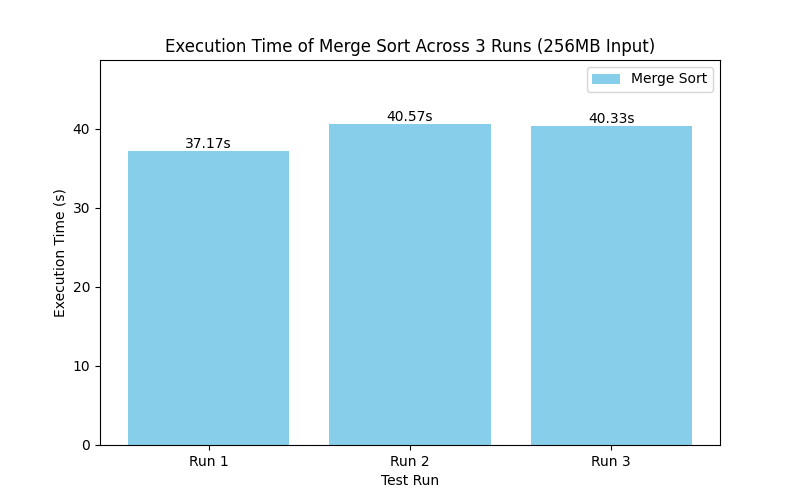
\includegraphics[width=\textwidth]{figures/merge_sort_time.png}
\caption{External Merge Sort runtime by merge degree $K$ (heuristic, 4, 8, 16) for the three 256~MB inputs.}
\label{fig:merge_sort_k_comparison}
\end{figure}

\begin{figure}[h!]
\centering
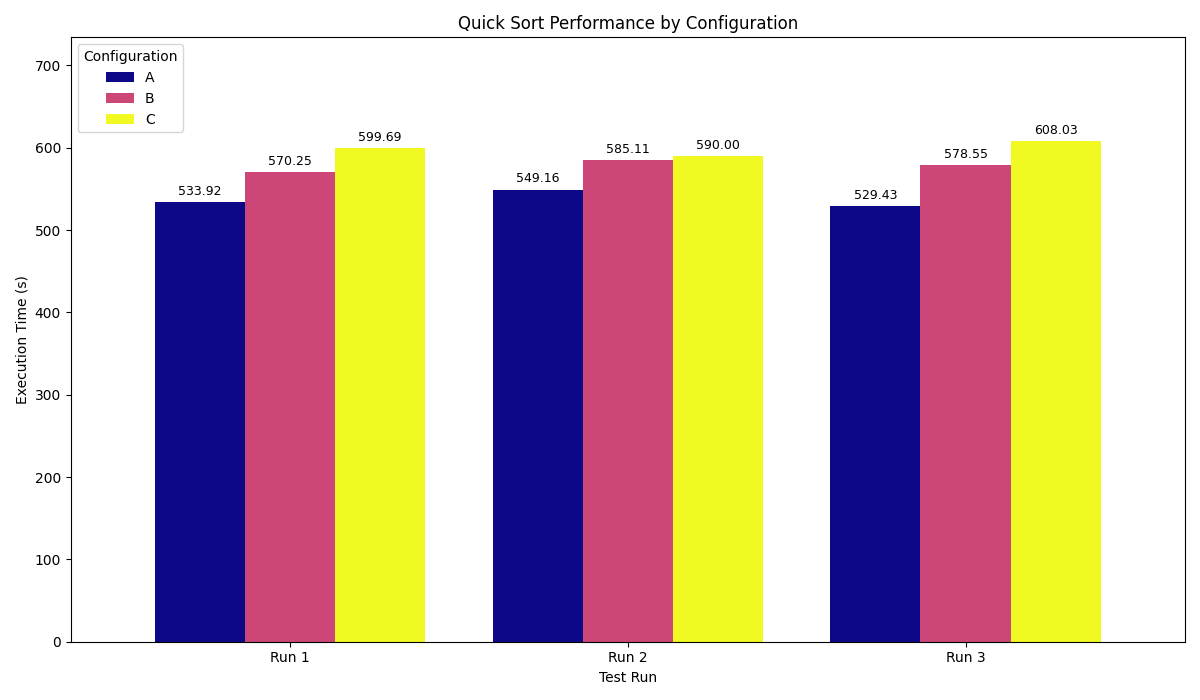
\includegraphics[width=\textwidth]{figures/quick_sort_time.png}
\caption{External Quick Sort runtime across buffer split configurations: QS\_A (2,2,2,10), QS\_B (1,1,1,13), QS\_C (2,1,1,12).}
\label{fig:quick_sort_config_comparison}
\end{figure}

\begin{figure}[h!]
\centering
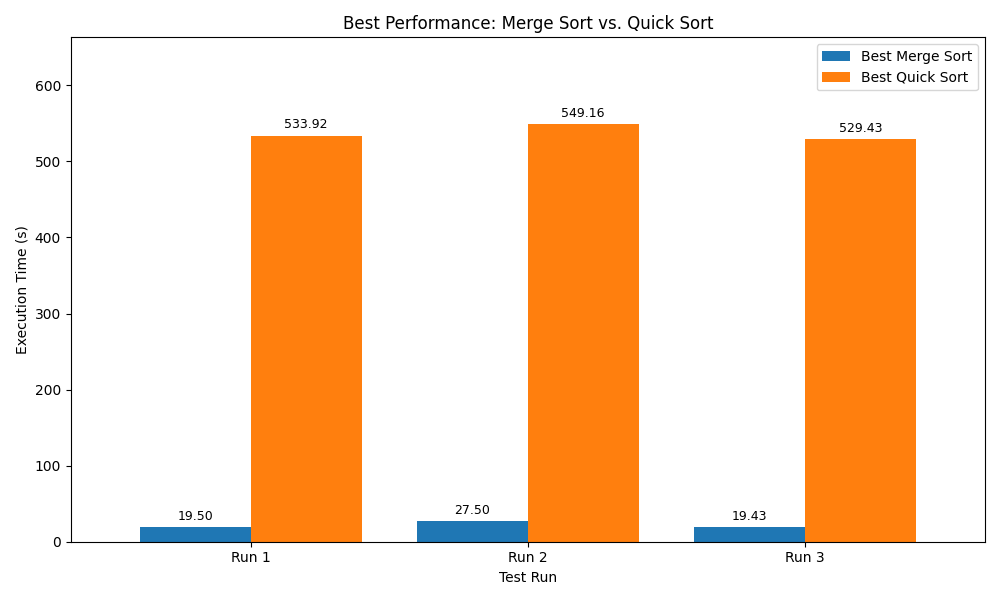
\includegraphics[width=0.8\textwidth]{figures/best_vs_best.png}
\caption{Best Merge Sort vs. Best Quick Sort per run (lowest time per algorithm per run).}
\label{fig:best_vs_best}
\end{figure}

\section*{Summary}
Varying $K$ in merge sort and adjusting the Input/Small/Large/Middle page splits in quick sort both have significant impact on execution time. Larger $K$ typically reduces the number of merge passes, while quick sort benefits from allocating a sufficiently large Middle buffer for the in-memory pivot window. The best-vs-best plot highlights the top performing configuration of each algorithm on the same inputs.
\end{document}
